% SVM parameter
\newcommand{\svmT}{\bm{\theta}}
\newcommand{\svmB}{b}
\newcommand{\svmAug}{\tilde{\svmT}}
%\newcommand{\svmAugAll}{\svmAug_{\text{all}}}
\newcommand{\svmAugAll}{\bm{\Theta}}

%\begin{figure}
%\begin{center}
%\subfigure[Early Adaptation]{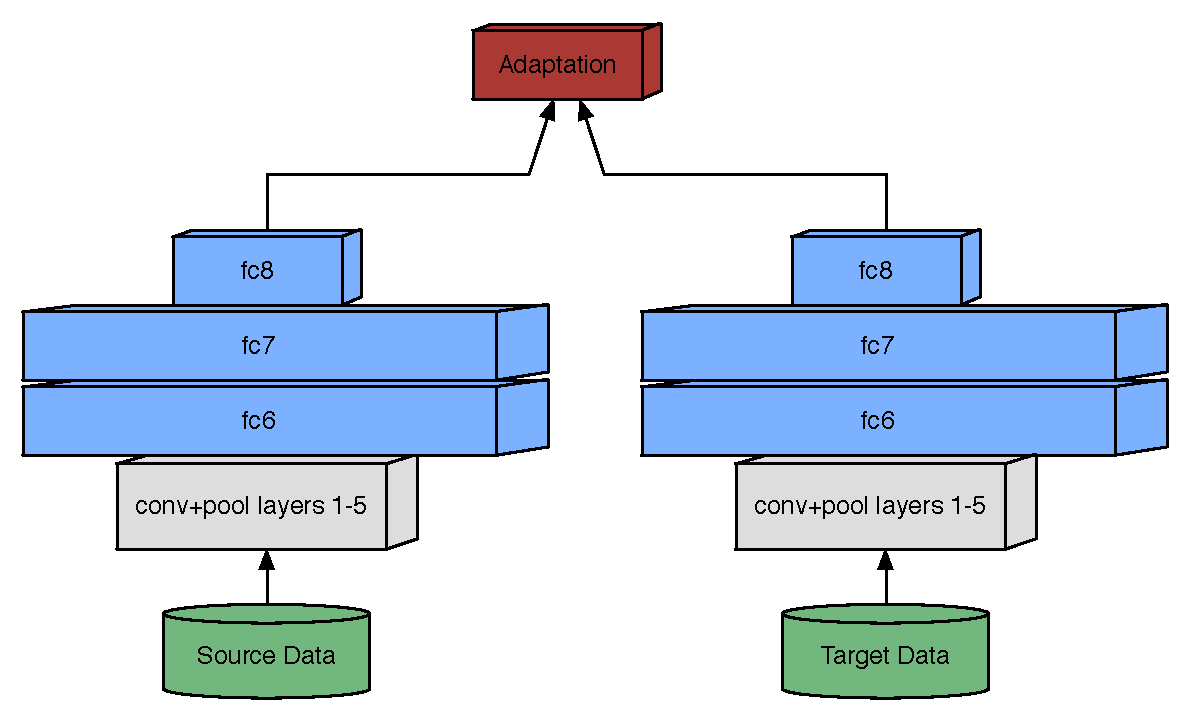
\includegraphics[width=.45\linewidth]{figs/model-adapt-unsuper}}
%\subfigure[Late Adaptation]{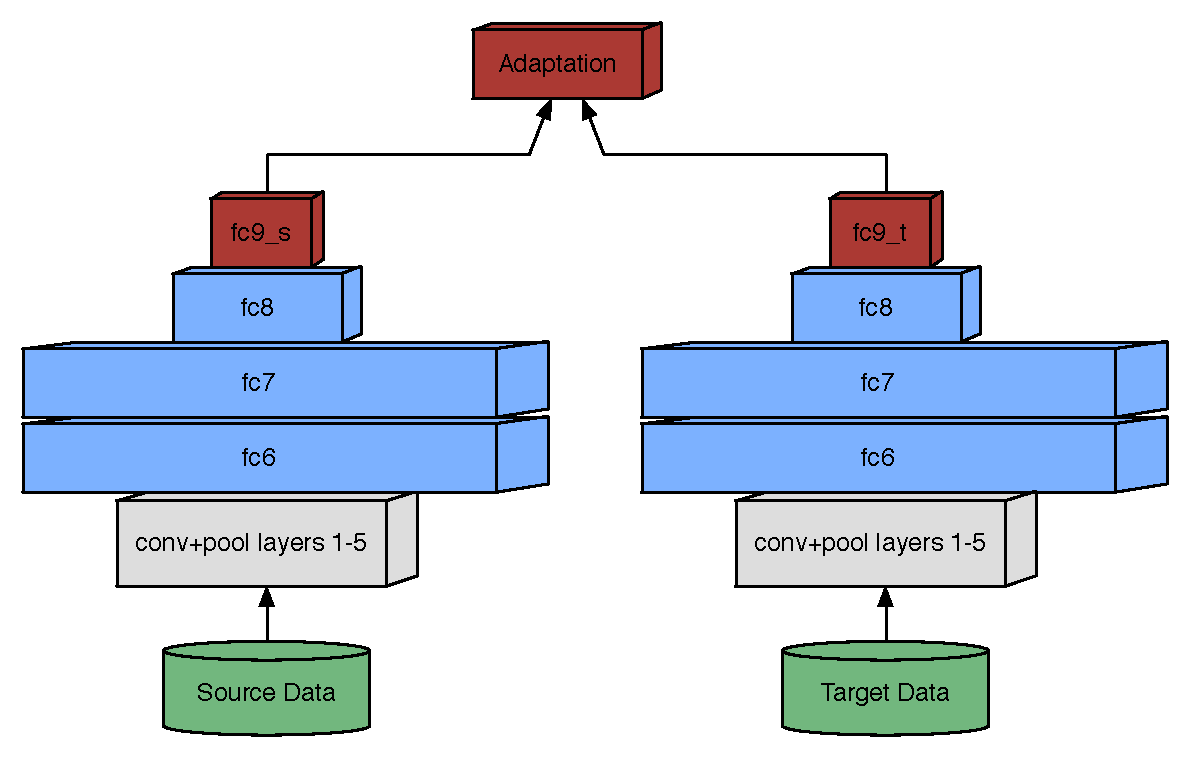
\includegraphics[width=.45\linewidth]{figs/model-adapt-super}}
%\end{center}
%\caption{Our proposed framework for adaptation. The source data and target data are each independently passed through the supervised convolutional neural network which has been trained on the 1.2Million images in the ILSVRC2012 Challenge dataset~\cite{ilsvrc2012}. We compute the subspace distance (A-distance) between the source and target data as it is represented in each of the fully connected layers of the network (represented in blue). The layer that produces the minimum subspace distance between source and target is chosen for adaptation. Finally, adaptation is performed on the activations from the best layer (shown in red).}
%\label{fig:model}
%\end{figure}

\begin{figure}
\begin{center}
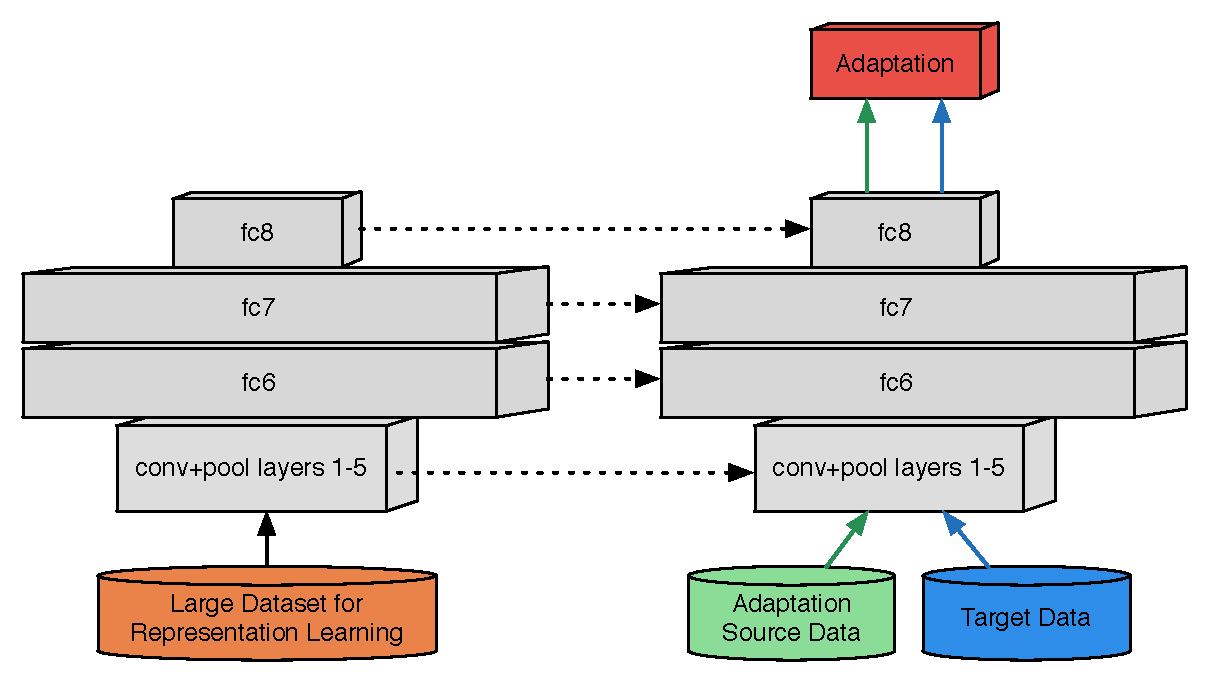
\includegraphics[width=.6\linewidth]{figs/model-adapt}
\end{center}
\caption{Our proposed framework for adaptation. We train a supervised CNN using a large labeled source dataset e.g. ImageNet, and use this to define the feature space. We then learn a model for use in the target domain by transferring the CNN parameters and training a new adaptation layer using the network activations for the source data and labeled (or unlabeled) target data.}
\label{fig:model-adapt}
\end{figure}

% Describe adaptation algorithms
%Many methods have been proposed for visual domain adaptation. 
% \ks{similar edit as in intro, see if this make sense}

We propose learning a supervised deep CNN using a large amount of
data from a relevant task to learn a representation. Then, we fix the network and train a new adaptation layer
that takes as input the activations from both the source and target data. By
using this hybrid approach we utilize the strong representation available from
the supervised deep model trained on a large source dataset while requiring only
enough target labeled data to train a shallow model with far fewer parameters.
%Here, we present a general framework for selectively adapting the parameters of a
%convolutional neural network (CNN) whose representation and classifier weights
%are trained on a large-scale source domain, such as ImageNet. 

We begin by training a supervised CNN using the architecture proposed by 
Krizhevsky et al~\cite{supervision}. This network has shown state of the art
performance for image classification and offers a strong starting model.
We fix the bottom-layer parameters in the
network and learn a single adaptation layer that takes as input
the activations from the fixed network for the target training data as well as an auxiliary labeled
dataset which is available to us at adaptation time (source data). The source data
can be (but isn't necessarily) the same data that was used to learn the representation.
This auxiliary source data will be used to adapt to the final target domain, and
provides more training examples than would otherwise be available from the limited target domain.

Figure~\ref{fig:model-adapt} illustrates our proposed framework for adapting a deep CNN
with limited target data. We depict the transfer of all pre-trained layers to the final adapted model
for simplicity of presentation,  however, in general, there is no reason to assume a priori that
adding the adaptation layer after all pre-trained layers is the best approach.

Intuitively, when selecting a layer to use for adaptation, we would like to use
the one in which the source and target appear the most similar (and thus
experience the least domain shift).
To select a layer, we assess the domain-invariance of each layer using their A-distances
\cite{adist}. A-distance is a measure of distance between two subspaces and hence 
can be used to measure the distinguishability of two datasets.

We compute the A-distance metric on the source and target activations after each fully 
connected layer
and automatically select the  layer after which
our source and target datasets are most similar, and hence most amenable to adaptation.

Given two domains $X_1$ and $X_2$, the A-distance between them is defined as:

\begin{equation}
  d_A(X_1, X_2) = 2 \left( 1 - 2 \min_{h' \in H} E(h'(X_1, X_2))\right)
\end{equation}


where $E(h^*(X_1, X_2))$ is the test error of the optimal hyperplane that attempts to
distinguish between the two domains.

In practice, it is NP-hard to find the optimal hyperplane, so we use a computationally simple and 
close approximation to the A-distance metric which was introduced by Ben-David et al~\cite{adist-comp}, 
where the optimal hyperplane is replaced by the classifier model parameter learned from a linear SVM.

Once we have selected which layer to use, we then add an adaptation layer above
the selected layer, as indicated in Figure~\ref{fig:model-adapt}. This layer
consists of an adaptation technique which combines the source and target
training data, then learns a linear classifier.

We explore three adaptation setups:
\begin{itemize}
  \item \textbf{Deep and Frustratingly Easy (DFE)}
    We first consider learning a joint layer directly over the source and target
    activations. For the semi-supervised setting, we choose to use a simple and
    surprisingly effective adaptation approach, proposed by \daume
    et al~\cite{daume}, that fits into our framework. It involves learning a
    single classifier model on an augmented feature space where there are source
    and target specific dimensions as well as a set of common dimensions.

  \item \textbf{Deep Late Fusion (DLF)}
    An alternative to DFE involves learning source and target specific
    adaptation layers independently and then learning an adaptation layer to
    combine them afterwards. One example adaptation approach that fits in the
    late fusion framework is to simply take a linear combination of the source
    and target output activations.

  \item \textbf{Deep Subspace Alignment (DSA)}
    For the unsupervised adaptation setting, we choose to use a recently
    proposed subspace alignment algorithm (SA)~\cite{sa}, which is applied to
    both the source and target activations before training a classification
    layer using just the available source data.

\end{itemize}

%We are interested in both unsupervised and supervised settings, so we examine
%two sets of adaptation techniques. For the unsupervised setting, we use the
%Geodesic Flow Kernel (GFK)~\cite{gong-cvpr12} and Subspace Alignment
%(SA)~\cite{sa} methods. For the supervised setting, we use the Late Fusion,
%\daume~\cite{daume}, Projective Model Transfer (PMT)~\cite{aytar-iccv11}, and
%Max-margin Domain Transforms (MMDT)~\cite{hoffman-iclr13} methods.
